\documentclass[a4paper]{article}

\usepackage[utf8]{inputenc}
\usepackage[portuges]{babel}
\usepackage{a4wide}
\usepackage{graphicx}
\usepackage{listings}
\usepackage{caption}
\usepackage{subcaption}
\title{Projeto de Programação Orientada aos Objetos\\Grupo 19}
\author{Henrique Pereira (a80261) \and Pedro Moreira (a82364) \and Pedro Ferreira (a81135) }




\begin{document}

\maketitle

\begin{figure}
\centering
\begin{subfigure}{.4\textwidth}
  \centering
  
\includegraphics[width=.3\linewidth]{henrique.png}
  \caption{Henrique Pereira}
\end{subfigure}
\begin{subfigure}{.4\textwidth}
  \centering
  
\includegraphics[width=.3\linewidth]{pedro.png}
  \caption{Pedro Moreira}
\end{subfigure}
\begin{subfigure}{.4\textwidth}
  \centering
  
\includegraphics[width=.3\linewidth]{ferreira.png}
  \caption{Pedro Ferreira}
\end{subfigure}
\end{figure}



\newpage

\tableofcontents

\newpage

\section{Introdução}
\label{sec:intro}

 No contexto da Unidade Curricular Programação Orientada aos Objetos (POO) foi proposto o desenvolvimento, na linguagem Java, da
 aplicação JAVA-Fatura. O enunciado proposto pelos docentes visa o desenvolvimento de uma versão da plataforma de disponibilização aos contribuintes
 da informação referente às faturas que foram emitidas em seu nome. Os requisitos básicos são, por exemplo, verificar as faturas 
 emitidas em seu nome, por parte do contribuinte individual, e obter o total faturado, por parte de uma empresa.
 Na seção \ref{sec:java} serão apresentados mais requisitos desta aplicação e também serão discutidas as classes 
 criadas para a concretização dos requisitos apresentados.
 Na seção \ref{sec:funcionalidades} será discutida a forma como um utilizador pode interagir com a aplicação.


\section{JAVA-Fatura}
\label{sec:java}

Para além dos requisitos já referidos, os contribuintes individuais devem ser capazes de verificar o montante de dedução fiscal acumulado (por si
e pelo agregado familiar), atribuir o setor de atividade económica a uma fatura que necessite, entre outros. As empresas deverão ser capazes de de obter
vários tipos de listagens sobre as faturas que emitiram, ordenadas por valor ou data. Para além disso, a aplicação necessita de ter um admistrador capaz 
de determinar os contribuintes que mais gastam no sistema ou de adicionar um novo setor de ativividade económica. Para a realização deste projeto, decidimos
criar as seguintes classes.	
	

%%%%%%%%%%%%%%%%%%%%%%%%%%%%%%%%%%%%%%%%%%%%%
\subsection{Classes}
\label{sec:classes}

Antes de iniciarmos a descrição de cada uma das classes, começamos por mostrar o seguinte diagrama das classes implementadas.

	% IMAGEM 
	
\subsubsection{BeneficioFiscal} %%%%%%%%%%%%%%%%%


Interface definida para que as famílias numerosas e as empresas do interior
terem um beneficio fiscal aquando da dedução das suas faturas.


\subsubsection{ConcelhosInterior} %%%%%%%%%%%%%%%

Classe que contém os concelhos que beneficiam de beneficio fiscal. MAIS!


\subsubsection{Contribuinte} %%%%%%%%%%%%%%%

Sendo subclasse de Entidade, esta classe tem a lista das faturas emitidas em seu nome (separadas pelas que são 
fiscalmente válidas ou inválidas), o número de dependentes familiares assim como os NIFs de toda a família.


\subsubsection{ContribuinteFamiliaNumerosa} %%%%%%%%%%%%%%%

Implementa a interface BeneficioFiscal. MAIS!


\subsubsection{Controller} %%%%%%%%%%%%%%%

Classe intermediária entre a comunicação do utilizador com o sistema. MAIS! 


\subsubsection{Distritos} %%%%%%%%%%%%%%%

Enum contendo todos os distritos do país.


\subsubsection{Empresa} %%%%%%%%%%%%%%%

Subclasse de Entidade que contém as faturas emitidas e os setores de atividade económica. MAIS!



\subsubsection{EmpresaInterior} %%%%%%%%%%%%%%%

Subclasse de Empresa que favorece de um benefício fiscal. MAIS! 


\subsubsection{Entidade} %%%%%%%%%%%%%%%

Classe que contém as informações básicas, como o nome e o email, assim como as credenciais necessárias para o log in (NIF e password)


\subsubsection{Fatura} %%%%%%%%%%%%%%%

Classe onde são guardadas as informações de cada fatura. MAIS!


\subsubsection{GestorSetor} %%%%%%%%%%%%%%%

Classe auxiliar à classe Fatura para que seja possível ao Contribuinte associar o setor de atividade económica que deseja à fatura em causa. 


\subsubsection{LogSetor} %%%%%%%%%%%%%%%

Classe auxiliar à classe GestorSetor que guarda o histórico de todas as alterações do setor de atividade económica que um contribuinte realizou.

 
\subsubsection{Menu} %%%%%%%%%%%%%%%

Classe que faz o display das operações que o utilizador pode realizar.


\subsubsection{Morada} %%%%%%%%%%%%%%%

NAO SEI XD


\subsubsection{Setor} %%%%%%%%%%%%%%%

Classe que contém as informações sobre a dedução relacionada com o setor de atividade económica.


\subsubsection{Sistema} %%%%%%%%%%%%%%%

Classe que guarda todas as informações da aplicação (dados de todas as entidades).



%%%%%%%%%%%%%%%%%%%%%%%%%%%%%%%%%%%%%%%%%%%%%
\subsection{Classes de Exceção}
\label{Casdads}

  \begin{itemize}
  	\item{AdminModeNaoAtivadoException - } 
    \item{ConcelhoNaoEInteriorException - } 
    \item{EntidadeAtivaNaoEEmpresaException - } 
    \item{NIFDaFaturaEEmpresaException - }
    \item{NIFJaRegistadoException - } 
    \item{NIFNaoEDeUmContribuinteException - }
    \item{NIFNaoRegistadoException - }
  \end{itemize}


%%%%%%%%%%%%%%%%%%%%%%%%%%%%%%%%%%%%%%%%%%%%%
\subsection{Decisões Tomadas}
\label{sec:decisoes}

Modelo MVC
GestorSetor



%%%%%%%%%%%%%%%%%%%%%%%%%%%%%%%%%%%%%%%%%%%%%
\subsection{Funcionalidades}
\label{sec:funcionalidades}

Qualquer utilizador quando inicia a aplicação é confrontado com o seguinte menu:

	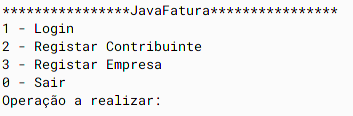
\includegraphics[width=.6\linewidth]{main_menu.png}

Caso o utilizador escolha efetuar o login (1) e o efetue com sucesso (mediante registo prévio no sistema)
o menu seguinte será diferente para cada uma das entidades apresentadas abaixo.
Ao registar, quer um contribuinte, quer uma empresa, serão pedidas informações relativas a cada uma das entidades.


\subsubsection{Contribuinte}

	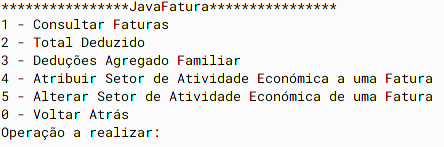
\includegraphics[width=.7\linewidth]{contribuinte_menu.png}


\subsubsection{Empresa}

	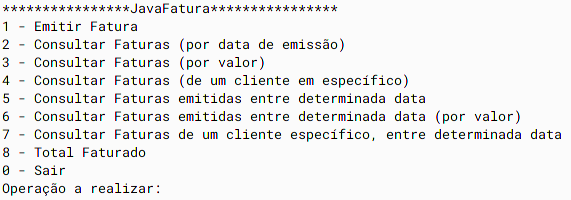
\includegraphics[width=.9\linewidth]{empresa_menu.png}


\subsubsection{Admistrador}

	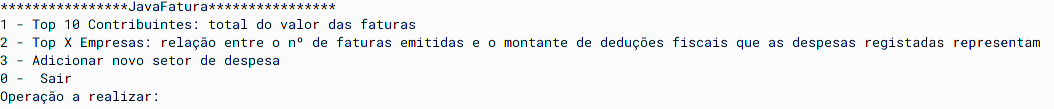
\includegraphics[width=.9\linewidth]{admin_menu.png}




\section{Conclusões}
\label{sec:conclusao}

Em suma, os requisitos propostos foram cumpridos e conjugados com êxito, sendo que o resultado final se revela um quanto fruitivo. 

Foi, no geral, um trabalho extremamente enriquecedor e altamente pedagógico uma vez que conjugou o trabalho cooperativo.

\end{document}\grid
